%-------------------------
% Resume in Latex
% Original author : Sourabh Bajaj
% Adaptation : Hyunggi Chang (changh95)
% License : MIT
%------------------------

\documentclass[letterpaper,11pt]{article}

\usepackage{latexsym}
\usepackage{kotex} % 한글 사용 가능! 
\usepackage[empty]{fullpage}
\usepackage{titlesec}
\usepackage{marvosym}
\usepackage[usenames,dvipsnames]{color}
\usepackage{verbatim}
\usepackage{enumitem}
\usepackage[hidelinks]{hyperref}
\usepackage{fancyhdr}
\usepackage[english]{babel}
\usepackage{tabularx}
\usepackage{booktabs}
\usepackage{amsmath}
\usepackage{tikz}
\usetikzlibrary{positioning, shapes.geometric, calc, backgrounds, arrows.meta}

\pagestyle{fancy}
\fancyhf{} % clear all header and footer fields
\fancyfoot{}
\renewcommand{\headrulewidth}{0pt}
\renewcommand{\footrulewidth}{0pt}

% Adjust margins
\addtolength{\oddsidemargin}{-0.5in}
\addtolength{\evensidemargin}{-0.5in}
\addtolength{\textwidth}{1in}
\addtolength{\topmargin}{-0.5in}
\addtolength{\textheight}{1.0in}

\urlstyle{same}

\raggedbottom
\raggedright
\setlength{\tabcolsep}{0in}

% Sections formatting
\titleformat{\section}{
  \vspace{-4pt}\scshape\raggedright\large
}{}{0em}{}[\color{black}\titlerule \vspace{-2pt}]

%-------------------------
% Custom commands - Do Look into this area, if you wish to customise further!
% 포맷이 마음에 들지 않으시다면 이 부분을 수정하세요!

\newcommand{\resumeItem}[1]{
  \item\small{
    {#1 \vspace{-2pt}}
  }
}

\newcommand{\resumeProject}[3]{
  \vspace{0pt}\item
    \begin{tabular*}{0.97\textwidth}[t]{l@{\extracolsep{\fill}}r}
      #1 & \small #2 \\
      {#3}
    \end{tabular*}\vspace{-5pt}
}

\newcommand{\resumeProjectNoDate}[2]{
  \vspace{0pt}\item
    #1 \\
    {#2}
    \vspace{-5pt}
}

\newcommand{\resumeSubProject}[2]{
  \item{
    {#1 \vspace{0pt}}
    {#2}
  }
}

\newcommand{\resumeSubheading}[4]{
  \vspace{-1pt}\item
    \begin{tabular*}{0.97\textwidth}[t]{l@{\extracolsep{\fill}}r}
      \textbf{#1} & \\
      \textit{\small#3} & \textit{\small #4} \\
    \end{tabular*}\vspace{-5pt}
}

\newcommand{\resumeSubItem}[2]{\resumeItem{#1}{#2}\vspace{-4pt}}

\renewcommand{\labelitemii}{$\circ$}

\newcommand{\resumeProjectListStart}{\begin{itemize}[leftmargin=*]}
\newcommand{\resumeProjectListEnd}{\end{itemize}}

\newcommand{\resumeSubProjectListStart}{\begin{itemize}[leftmargin=*]}
\newcommand{\resumeSubProjectListEnd}{\end{itemize}}

\newcommand{\resumeSubHeadingListStart}{\begin{itemize}[leftmargin=*]}
\newcommand{\resumeSubHeadingListEnd}{\end{itemize}}
\newcommand{\resumeItemListStart}{\begin{itemize}}
\newcommand{\resumeItemListEnd}{\end{itemize}\vspace{-5pt}}

%-------------------------------------------
%%%%%%  CV STARTS HERE  %%%%%%%%%%%%%%%%%%%%%%%%%%%%


\begin{document}

%----------HEADING-----------------
\begin{tabular*}{\textwidth}{l@{\extracolsep{\fill}}r}
  \textbf{\Large 경력 기술서} & Github: superhuman54 \\
  \href{https://superhuman54.github.io}{https://superhuman54.github.io} & Email : \href{mailto:YourEmail@gmail.com}{superhuman54.tech@gmail.com} \\
  {} & Mobile : (+82) 010-4691-0485
\end{tabular*}

%-----------PROJECTS-----------------
\section{\textbf{1. 액션로그 파이프라인}}
  \resumeProjectListStart
    \resumeProject
    {\textbf{소속}: 드림어스컴퍼니} {}
    
    {\textbf{주요 내용}}:
    
    액션로그 파이프라인 프로젝트는 대규모 로그 데이터(하루 3억건)를 신속하고 안정적으로 수집·처리·분석하기 위한 End-to-End 데이터 파이프라인을 구축하고 운영한 경험을 담고 있습니다. Kafka와 Amazon Glue Crawler 기반의 실시간 데이터 처리, S3 및 Amazon Glue를 이용한 데이터 레이크 구축, Airflow를 활용한 데이터 적재 작업 자동화와 운영 모니터링, 그리고 효율적인 파티션 설계를 통한 대용량 ETL 작업의 성능 최적화까지 다양한 데이터 엔지니어링 과제 전반을 맡아 수행했습니다.

    \vspace{3mm}
    
    \resizebox{0.95\textwidth}{!}{ % 95% 너비로 자동 축소
    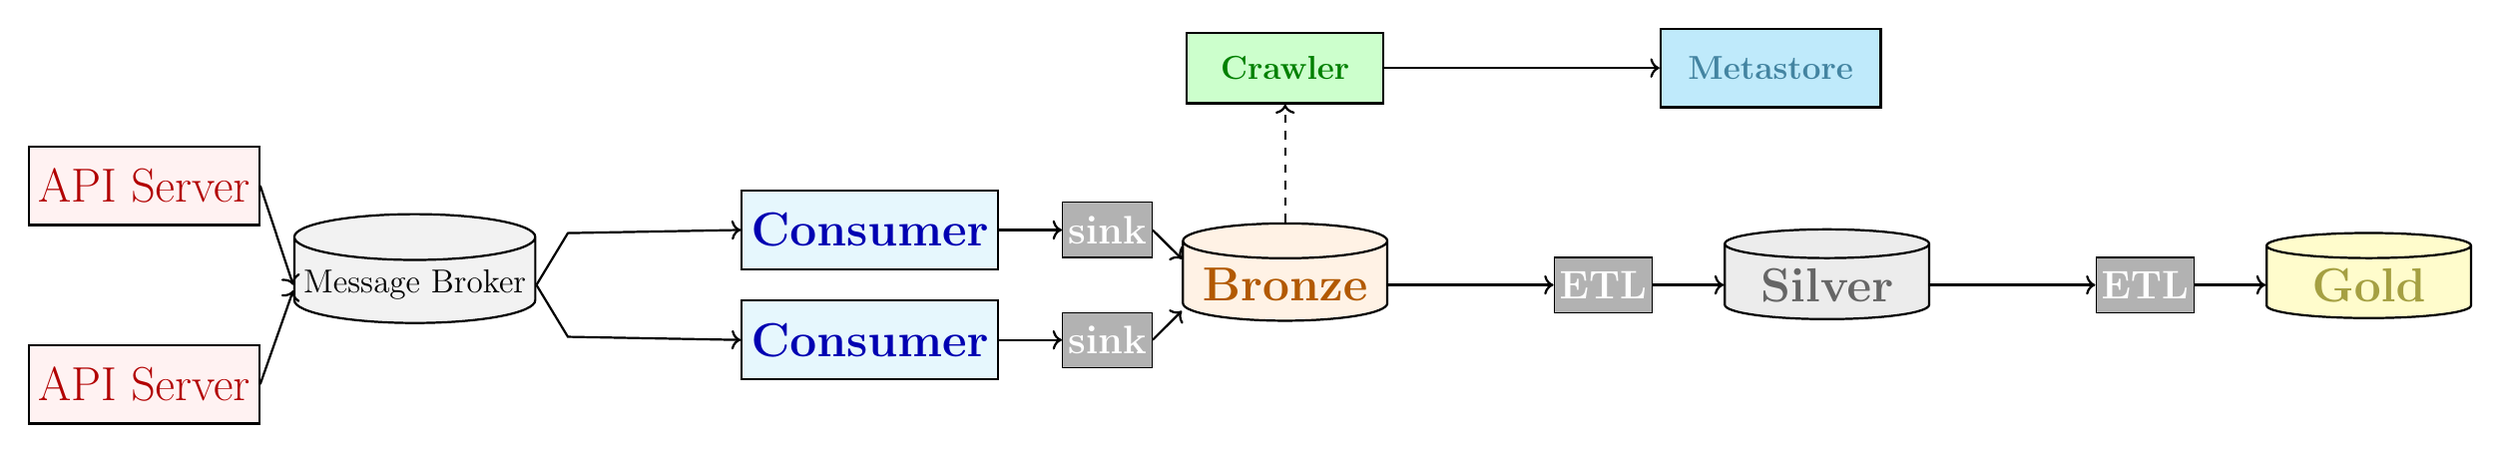
\begin{tikzpicture}[
        font=\sffamily,
        % 노드 스타일
        apiServer/.style={
            draw,
            rectangle,
            minimum width=2.8cm,
            minimum height=1.0cm,
            thick,
            fill=red!5!white,
            text=red!70!black,
            font=\LARGE,
        },
        broker/.style={
            draw,
            cylinder,
            shape border rotate=90,
            aspect=0.19,
            minimum width=2.6cm,
            minimum height=1.0cm,
            thick,
            fill=gray!10,
            font=\large
        },
        consumer/.style={
            draw,
            rectangle,
            minimum width=2.8cm,
            minimum height=1.0cm,
            thick,
            fill=cyan!10,
            font=\LARGE\bfseries,
            text=blue!70!black
        },
        graybox/.style={
            draw,
            fill=gray!60,
            minimum width=1.1cm,
            minimum height=0.7cm,
            text=white,
            font=\bfseries\Large,
            inner sep=2pt
        },
        bronze/.style={
            draw,
            cylinder,
            shape border rotate=90,
            aspect=0.19,
            minimum width=2.6cm,
            minimum height=1.0cm,
            thick,
            fill=orange!10,
            font=\LARGE\bfseries,
            text=orange!70!black
        },
        silver/.style={
            draw,
            cylinder,
            shape border rotate=90,
            aspect=0.19,
            minimum width=2.6cm,
            minimum height=1.0cm,
            thick,
            fill=gray!15,
            font=\LARGE\bfseries,
            text=gray!80!black
        },
        gold/.style={
            draw,
            cylinder,
            shape border rotate=90,
            aspect=0.19,
            minimum width=2.6cm,
            minimum height=1.0cm,
            thick,
            fill=yellow!20,
            font=\LARGE\bfseries,
            text=yellow!60!black
        },
        crawler/.style={
            draw,
            rectangle,
            minimum width=2.5cm,
            minimum height=0.9cm,
            fill=green!20,
            thick,
            font=\large\bfseries,
            text=green!50!black
        },
        catalog/.style={
            draw,
            rectangle,
            minimum width=2.8cm,
            minimum height=1.0cm,
            fill=cyan!25,
            thick,
            font=\large\bfseries,
            text=cyan!60!black
        },
        myarrow/.style={thick,->}
    ]
    
    % 1. API Servers
    \node[apiServer] (API1) at (0,0.8) {API Server};
    \node[apiServer, below=1.5cm of API1] (API2) {API Server};
    
    % 2. Message Broker
    \node[broker, right=1.9cm of $(API1)!0.5!(API2)$] (MB) {Message Broker};
    
    % 3. Consumers
    \node[consumer, right=2.6cm of MB, yshift=0.7cm] (C1) {Consumer};
    \node[consumer, right=2.6cm of MB, yshift=-0.7cm] (C2) {Consumer};
    
    % 4. sink gray boxes  
    \node[graybox, right=0.8cm of C1] (sink1) {sink};
    \node[graybox, right=0.8cm of C2] (sink2) {sink};
    
    % 5. Bronze S3
    \node[bronze, right=0.95cm of $(sink1)!0.5!(sink2)$] (Bronze) {Bronze};
    
    % 6. ETL gray box
    \node[graybox, right=2.1cm of Bronze] (ETL1) {ETL};
    \node[silver, right=0.9cm of ETL1] (Silver) {Silver};
    \node[graybox, right=2.1cm of Silver] (ETL2) {ETL};
    \node[gold, right=0.9cm of ETL2] (Gold) {Gold};
    
    % 7. Glue Crawler and Glue Catalog, placed above Bronze
    \node[crawler, above=1.5cm of Bronze] (Crawler) {Crawler};
    \node[catalog, right=3.5cm of Crawler] (Catalog) {Metastore};
    
    % --- edges
    % API Servers to Broker
    \draw[myarrow] (API1.east) -- (MB.west);
    \draw[myarrow] (API2.east) -- ([yshift=-2pt]MB.west);
    
    % Broker to Consumers
    \draw[myarrow] (MB.east) -- ++(0.4,0.66) -- (C1.west);
    \draw[myarrow] (MB.east) -- ++(0.4,-0.66) -- (C2.west);
    
    % Consumers to sink box to Bronze
    \draw[myarrow] (C1.east) -- (sink1.west); 
    \draw[myarrow] (sink1.east) -- ($(Bronze.west)+(0,0.33)$);
    \draw[myarrow] (C2.east) -- (sink2.west); 
    \draw[myarrow] (sink2.east) -- ($(Bronze.west)+(0,-0.33)$);
    
    % Bronze -> ETL1 -> Silver -> ETL2 -> Gold
    \draw[myarrow] (Bronze.east) -- (ETL1.west);
    \draw[myarrow] (ETL1.east) -- (Silver.west);
    \draw[myarrow] (Silver.east) -- (ETL2.west);
    \draw[myarrow] (ETL2.east) -- (Gold.west);
    
    % Glue Crawler -> Glue Catalog
    \draw[myarrow] (Crawler.east) -- (Catalog.west);
    
    % Glue Crawler -> Bronze (partition discovery)
    \draw[myarrow,dashed] (Bronze.north) -- (Crawler.south);
    
    \end{tikzpicture}
    }

    \vspace{3mm}

    % ------------- 다이어그램 End
    
    \textbf{주요 성과}:
        
\begin{itemize}
    \item ETL 파이프라인 자동화 및 준실시간 탐색을 위한 크롤러 구축
\end{itemize}
\begin{itemize}
    \item S3 파티션 구조와 적재 정책을 최적화하여, 소규모 파일 문제를 해결하고 파티션 단위 처리 효율을 높여 Bronze에서 Silver로 ETL 처리하는 구간의 전체 작업 시간을 평균 약 35\% (22분 → 15분) 감축하였습니다.
\end{itemize}

    \resumeSubProjectListStart
        \resumeSubProject {\textbf{메달리온 아키텍쳐 설계}}
        {
        
        메달리온 아키텍처를 적용하여 로그 데이터를 여러 단계로 분리 및 정제함으로써, 데이터 품질과 신뢰성을 체계적으로 개선하였습니다. 원시 데이터 보존을 통해 언제든 재처리가 가능하고, 각 단계별 데이터 검증과 정합성 보장을 통해 오류 데이터는 낮은 단계에 격리하여 상위 단계에서는 정확하고 고품질 데이터를 확보하였습니다. 이로써 분석과 비즈니스 활용에 최적화된 신뢰성 높은 데이터 환경을 구축하였습니다.
        % 원시 데이터(Raw, Bronze) → 정제 데이터(Clean, Silver) → 고품질 데이터(Gold)로 계층화하여
        % 오류나 결함이 있는 데이터는 낮은 단계에 가두고, 상위 단계에서는 깨끗한 데이터만 사용함으로써 품질 보장함.

        \vspace{1mm}
        \textbf{사용한 기술}: Amazon S3, Amazon Glue Data Catalog, Kafka Connect, Apache Spark
        \vspace{2mm}
        }
        \resumeSubProject {\textbf{데이터 수집 및 처리 최적화}}
        
        {
        대용량 액션로그 데이터를 수집하기 위해 Kafka 기반의 스트리밍 플랫폼을 구축하고, Amazon Glue Crawler로 준실시간 파티션 등록과 Spark 배치 처리를 병행하는 하이브리드 아키텍처를 설계했습니다.

        \vspace{1mm}
        \textbf{사용한 기술}: Apache Spark, Amazon Glue Crawler
        \vspace{2mm}
    }
    \resumeSubProject{\textbf{파티션 크기 조정 및 ETL 성능 개선}}
    {
    S3에 저장되는 로그 데이터의 파티션 크기를 효율적으로 튜닝하여 Spark 처리 시 불필요한 소규모 파일 생성을 획기적으로 줄였고, 파티션의 파일 수를 적정 수준으로 유지함으로써 job당 입력 스캔 비용을 절감하였습니다. 그 결과, 전체 ETL 파이프라인 수행 시간이 평균 35\% (22분 → 15분) 단축되었습니다.

        \vspace{1mm}
        \textbf{사용한 기술}: PySpark, Python
        \vspace{2mm}
    }
    \resumeSubProjectListEnd
  \resumeProjectListEnd

%-------------------------------------------
\section{\textbf{2. 침해곡 탐지 파이프라인}}
  \resumeProjectListStart
    \resumeProject
    {\textbf{소속}: 드림어스컴퍼니} {}
    
    {\textbf{주요 내용}}:
    
    유통사에서 신규로 입수되는 오디오(하루 7만$\sim$16만 곡)를 FLO 플랫폼 내 500만 곡 보호 음원과 자동 비교해 침해곡(동일·변조곡)을 판별하는 대규모 파이프라인입니다. 파이프라인은 주기적으로 대규모 신규 데이터를 사전 처리하고, 임베딩 추출과 벡터 유사도 연산 단계를 시스템입니다. 과거 파이썬 기반 배치 시스템의 한계를 극복하고자, 데이터프레임 처리 엔진으로 Polars를 도입해 I/O 병목과 실행 비용을 크게 개선했습니다. 또한 벡터 데이터베이스 적용을 통해 수백만 곡 임베딩 간 유사도 필터링(코사인 거리 등) 처리 속도를 대폭 향상시켰으며, 전체 탐지 파이프라인의 정확도와 운영 효율이 올라갔습니다.

    \vspace{3mm}

    \resizebox{0.95\textwidth}{!}{
        \begin{tikzpicture}[
            font=\sffamily,
            apiServer/.style={
                draw,
                rectangle,
                minimum width=2.9cm,
                minimum height=1.0cm,
                thick,
                fill=cyan!8,
                font=\large,
                align=center,
                text=black,
            },
            s3box/.style={
                draw,
                cylinder,
                shape border rotate=90,
                aspect=0.19,
                minimum width=2.1cm,
                minimum height=1.05cm,
                thick,
                fill=magenta!10,
                font=\Large,
                text=magenta!70!black,
                align=center,
            },
            vectordb/.style={
                draw,
                cylinder,
                shape border rotate=90,
                aspect=0.26,
                minimum width=2.4cm,
                minimum height=1.2cm,
                thick,
                fill=violet!10,
                font=\Large,
                text=violet!80!black,
                align=center,
            },
            notifbox/.style={
                draw,
                rectangle,
                thick,
                rounded corners=4pt,
                minimum width=2.9cm,
                minimum height=1.05cm,
                fill=green!13,
                font=\Large,
                text=green!40!black,
                align=center,
            },
            labelbox/.style={
                draw,
                rectangle,
                minimum width=0.95cm,
                minimum height=0.68cm,
                fill=gray!60,
                text=white,
                font=\bfseries,
                inner sep=2pt,
                align=center,
            },
            mysql/.style={
                draw,
                cylinder,
                shape border rotate=90,
                aspect=0.19,
                minimum width=2.1cm,
                minimum height=1.0cm,
                thick,
                fill=purple!20,
                font=\Large,
                text=purple!70!black,
                align=center,
            },
            cdn/.style={
                draw,
                rectangle,
                thick,
                minimum width=3cm,
                minimum height=1cm,
                fill=yellow!20,
                font=\large,
                align=center,
            },
            arr/.style={thick,->},
            dasharr/.style={thick,dashed,->,color=gray!70},
            node distance=0.4cm and 0.3cm
        ]
        
        % MySQL 노드 (추가)
        \node[mysql] (MySQL) at (0,0) {MySQL};
        
        % Preprocess 노드
        \node[apiServer, right=2.5cm of MySQL] (PP) {Preprocess};
        
        % 오디오 ID Read 라벨
        \node[labelbox, above=0.35cm of $(MySQL)!0.5!(PP)$] (readId) {read audioID};
        
        % S3 노드(첫번째)
        \node[s3box, right=2.3cm of PP] (S3A) {S3};
        
        % Embedding Extract 노드
        \node[apiServer, right=2.3cm of S3A] (EE) {Embedding\\Extract};
        
        % CDN 서버 노드 (서브 브랜치, 아래에)
        \node[cdn, below=1.5cm of EE] (CDN) {CDN Server};
        
        % Vector DB
        \node[vectordb, right=2.3cm of EE] (VDB) {Vector DB};
        
        % Filter
        \node[apiServer, right=2.3cm of VDB] (F) {Filter};
        
        % 두번째 S3 노드
        \node[s3box, right=2.3cm of F] (S3B) {S3};
        
        % Compile 노드
        \node[apiServer, right=2.3cm of S3B] (C) {Compile};
        
        % Slack Notify 노드
        \node[notifbox, right=2.3cm of C] (SN) {Slack Notify};
        
        % 라벨링
        \node[labelbox, above=0.32cm of $(PP)!0.5!(S3A)$] (l1) {write};
        \node[labelbox, above=0.32cm of $(S3A)!0.5!(EE)$] (l2) {read};
        \node[labelbox, right=0.2cm of $(EE)!0.5!(CDN)$] (l3) {download AAC};
        \node[labelbox, above=0.32cm of $(EE)!0.5!(VDB)$] (l4) {write};
        \node[labelbox, above=0.32cm of $(VDB)!0.5!(F)$] (l5) {read};
        \node[labelbox, above=0.32cm of $(F)!0.5!(S3B)$] (l6) {write};
        \node[labelbox, above=0.32cm of $(S3B)!0.5!(C)$] (l7) {read};
    
        
        % 수평 화살표
        \draw[arr] (MySQL.east) -- (PP.west);
        \draw[arr] (PP.east) -- (S3A.west);
        \draw[arr] (S3A.east) -- (EE.west);
        \draw[arr] (EE.east) -- (VDB.west);
        \draw[arr] (VDB.east) -- (F.west);
        \draw[arr] (F.east) -- (S3B.west);
        \draw[arr] (S3B.east) -- (C.west);
        \draw[arr] (C.east) -- (SN.west);
        
        % CDN 분기 화살표 (Embedding Extract → CDN)
        \draw[arr] (EE.south) -- (CDN.north);
        
        % CDN → Embedding Extract (다운로드 후 리턴)
        % \draw[arr] (CDN.east) .. controls +(right:8mm) and +(down:6mm) .. (EE.south east);

        \end{tikzpicture}
    
    }
    \vspace{3mm}
    \textbf{주요 성과}:
    
    \begin{itemize}
        \item 대규모 500만 곡 데이터 환경에서 Polars와 벡터 데이터베이스를 적용하여 동/변조곡 탐지 정확도가 18\%p(5\% $\rightarrow$ 23\%) 향상
        \item Polars 기반 고성능 배치 처리와 Kubernetes 리소스 최적화로, 하루 운영 비용이 약 73\%(\$12.4 $\rightarrow$ \$3.3, EC2 기준) 절감
        \item 벡터 연산 및 데이터 처리 효율 극대화로, 레포트 출력까지 소요 시간이 14시간에서 평균 6.5시간으로 53\% 단축
    \end{itemize}
%     \begin{table}[ht]
% \centering

% \begin{tabularx}{\textwidth}{X c c}
% \toprule
% \textbf{성과 항목} & \textbf{절대 향상/절감} & \textbf{기존 $\rightarrow$ 개선} \\
% \midrule
% 대규모 500만 곡 환경에서 Polars 및 벡터 데이터베이스 적용으로 탐지 정확도 향상 & +18\,\%p & 5\,\% $\rightarrow$ 23\,\% \\
% Polars 기반 배치 처리 및 Kubernetes 리소스 최적화로 하루 운영 비용 절감 & –73\,\% & \$12.4 $\rightarrow$ \$3.3 \\
% 벡터 연산 및 데이터 처리 효율 극대화로 레포트 출력 시간 단축 & –53\,\% & 14\,h $\rightarrow$ 6.5\,h \\
% \bottomrule
% \end{tabularx}
% \end{table}

    
    \resumeSubProjectListStart
        \resumeSubProject {\textbf{대규모 오디오 벡터 유사도 비교 처리속도 향상}}
        {
        
        신규로 유입되는 수만~수십만 곡의 오디오와 500만 곡 규모의 보호음원 간 임베딩 기반 유사도(코사인 거리) 비교를 자동화하였고, 이벤트 기반 워커 아키텍처 및 벡터 데이터베이스(PostgreSQL) 도입으로 병렬 연산 처리량을 극대화했습니다.
        
        \vspace{1mm}
        \textbf{사용한 기술}: Python, TensorFlow, PostgreSQL, asyncio
        \vspace{2mm}
        }
        \resumeSubProject {\textbf{Polars 기반 파이프라인 리뉴얼 및 운영 효율화}}
        {
        
        레거시 파이썬 기반 데이터프레임 처리 시스템을 Rust+SIMD가 적용된 Polars 엔진으로 전환하여, 대용량 Parquet 데이터 처리 시간과 I/O 병목을 획기적으로 줄이고, 전체 파이프라인의 실행 비용과 리포트 출력 시간을 크게 단축시켰습니다.
    
        \vspace{1mm}
        \textbf{사용한 기술}: Python, Polars, Kubernetes(Amazon EKS), Amazon S3
        \vspace{2mm}
        }
    \resumeSubProjectListEnd
  \resumeProjectListEnd

%-------------------------------------------
\section{\textbf{3. \href{https://trino.io/}{Trino} 구축 및 운영}}
  \resumeProjectListStart
    \resumeProject
    {\textbf{소속}: 드림어스컴퍼니} {}
    
    {\textbf{주요 내용}}:
    
    대규모 전사 멀티테넌트 데이터 플랫폼의 쿼리 엔진으로 Amazon EMR 기반 Presto를 사용하다가, Trino로 전환하는 프로젝트를 주도했습니다. 전환하면서 마주쳤던 다양한 문제를 해결하고, 쿼리 속도를 개선하였습니다.

    %---------------- 주요 내용 End

    \vspace{3mm}
\begin{figure}[ht]
    \centering
   \resizebox{0.70\textwidth}{!}{
        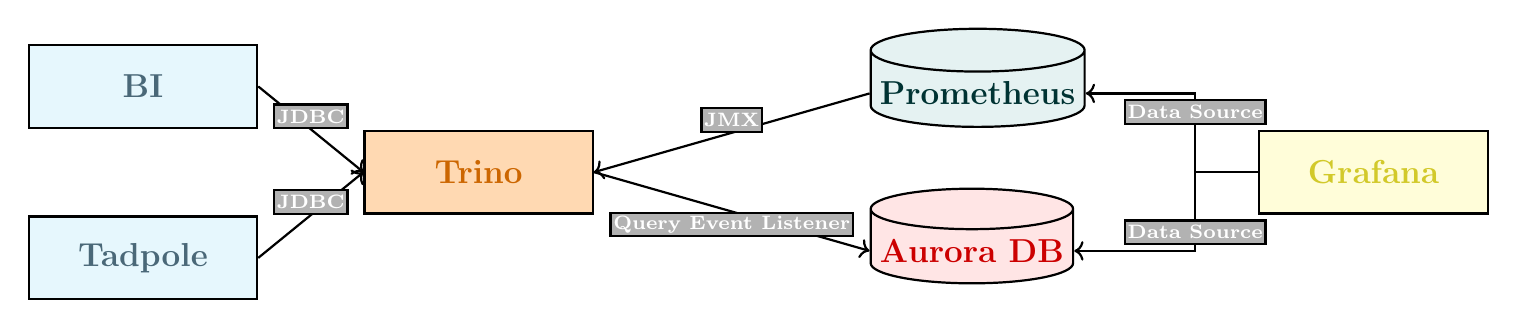
\begin{tikzpicture}[
    font=\sffamily,
    smallblock/.style={
        draw,
        rectangle,
        minimum width=2.9cm,
        minimum height=1.05cm,
        thick,
        fill=orange!30,
        font=\large\bfseries,
        align=center,
        text=orange!80!black
    },
    blueblock/.style={
        draw,
        rectangle,
        minimum width=2.9cm,
        minimum height=1.05cm,
        thick,
        fill=cyan!10,
        font=\large\bfseries,
        align=center,
        text=cyan!40!black
    },
    tealblock/.style={
        draw,
        cylinder,
        shape border rotate=90,
        aspect=0.20,
        minimum width=2.3cm,
        minimum height=1.05cm,
        thick,
        fill=teal!10,
        font=\large\bfseries,
        align=center,
        text=teal!40!black
    },
    redcylinder/.style={
        draw,
        cylinder,
        shape border rotate=90,
        aspect=0.20,
        minimum width=2.3cm,
        minimum height=1.05cm,
        thick,
        fill=red!10,
        font=\large\bfseries,
        align=center,
        text=red!80!black
    },
    beigeblock/.style={
        draw,
        rectangle,
        minimum width=2.9cm,
        minimum height=1.05cm,
        thick,
        fill=yellow!15,
        font=\large\bfseries,
        align=center,
        text=yellow!80!black
    },
    labelbox/.style={
        draw,
        rectangle,
        minimum width=0.6cm,
        minimum height=0.3cm,
        fill=gray!60,
        text=white,
        font=\scriptsize\bfseries,
        inner sep=1pt,
        align=center
    },
    arr/.style={thick,->},
    node distance=1.1cm and 1.5cm
]
% 노드들 위치 지정
\node[blueblock] (bi) at (0, 0.7) {BI};
\node[blueblock, below=1.1cm of bi] (tadpole) {Tadpole};
\node[smallblock, right=2.8cm of $(bi)!0.5!(tadpole)$] (trino) {Trino};
\node[tealblock, right=3.5cm of trino, yshift=1.0cm] (prom) {Prometheus};
\node[redcylinder, right=3.5cm of trino, yshift=-1.0cm] (aurora) {Aurora DB};
\node[beigeblock, right=3.6cm of $(prom)!0.5!(aurora)$] (grafana) {Grafana};
% 화살표와 라벨 (수직/수평선만 사용)
\draw[arr] (bi.east) -- node[labelbox, above] {JDBC} (trino.west);
\draw[arr] (tadpole.east) -- node[labelbox, above] {JDBC} (trino.west);
\draw[arr] (prom.west) -- node[labelbox, above] {JMX} (trino.east);
\draw[arr] (trino.east) -- node[labelbox, below] {Query Event Listener} (aurora.west);
% Grafana -> Prometheus (ㄱ자 경로)
\draw[arr] (grafana.west) -- ++(-0.8,0) |- node[labelbox, above, pos=0.3] {Data Source} (prom.east);
% Grafana -> Aurora DB (ㄱ자 경로)  
\draw[arr] (grafana.west) -- ++(-0.8,0) |- node[labelbox, below, pos=0.3] {Data Source} (aurora.east);
\end{tikzpicture}        
        
    }
\end{figure}
    \vspace{3mm}
    
    \textbf{주요 성과}:
        \begin{itemize}
            \item Presto에서 Trino로의 전환을 성공적으로 완료하여, 쿼리 처리 속도 15\% 증가
            \item 전환 과정에서 발생한 다양한 운영 이슈를 체계적으로 해결하여, 멀티테넌트 환경에서의 안정적인 서비스 제공 기반을 구축
        \end{itemize}

    %---------------- 주요 성과 End

    \resumeSubProjectListStart
        \resumeSubProject {\textbf{Observability 강화를 위한 모니터링 구축}}
        {
        
        Trino 클러스터 운영의 효율성을 높이고 실시간 성능 모니터링과 장애 대응을 위해 Prometheus와 Grafana 기반의 통합 모니터링 시스템을 구축하였습니다. 이를 통해 쿼리 성능, 자원 사용 현황 등 다양한 메트릭을 시각화하고, 멀티테넌트 환경에서 발생할 수 있는 다양한 문제들에 대해 신속히 탐지 및 대응할 수 있는 체계를 마련하였습니다. 이 모니터링으로 인해 느린 쿼리 발견하고 해결하였습니다.

        \vspace{1mm}
        \textbf{사용한 기술}: Prometheus, Grafana, MySQL, Python
        \vspace{2mm}
        }
    \resumeSubProjectListEnd

    %---------------- 서브 프로젝트 End

    \textbf{문제 해결(링크)}:
        \begin{itemize}
            \item \href{https://superhuman54.github.io/posts/trino-outofmemory/}{Trino 메모리 누수: Hadoop FileSystem Cache의 함정}
            \item \href{https://superhuman54.github.io/posts/trino-slow-query-analysis/}{Trino 느린 쿼리 분석과 성능 최적화}
        \end{itemize}
    
    %---------------- 트러블슛 End
    
  \resumeProjectListEnd

%-------------------------------------------
\section{\textbf{4. Amazon S3 기반 데이터레이크, 데이터웨어하우스 운영}}
  \resumeProjectListStart
    \resumeProject
    {\textbf{소속}: 드림어스컴퍼니} {}
    
    {\textbf{주요 내용}:

    FLO 서비스에서 사용하는 RDBMS, MongoDB, 로그, 지표를 저장하는 데이터레이크와 데이터웨어하우스를 운영하고, Spark on Amazon EMR, Amazon Glue Data Catalog로 필요한 데이터마트를 구성하였습니다. 또한, Airflow(Amazon MWAA)를 활용해 데이터 파이프라인 스케줄링 자동화를 구현하고, 클라이언트로 Kubernetes(Amazon EKS)를 사용하여 Amazon EMR과 상호작용하며 리소스 활용도와 운영 효율을 극대화하였습니다.

    \vspace{3mm}
    \begin{figure}[ht]
    \centering
   \resizebox{0.50\textwidth}{!}{
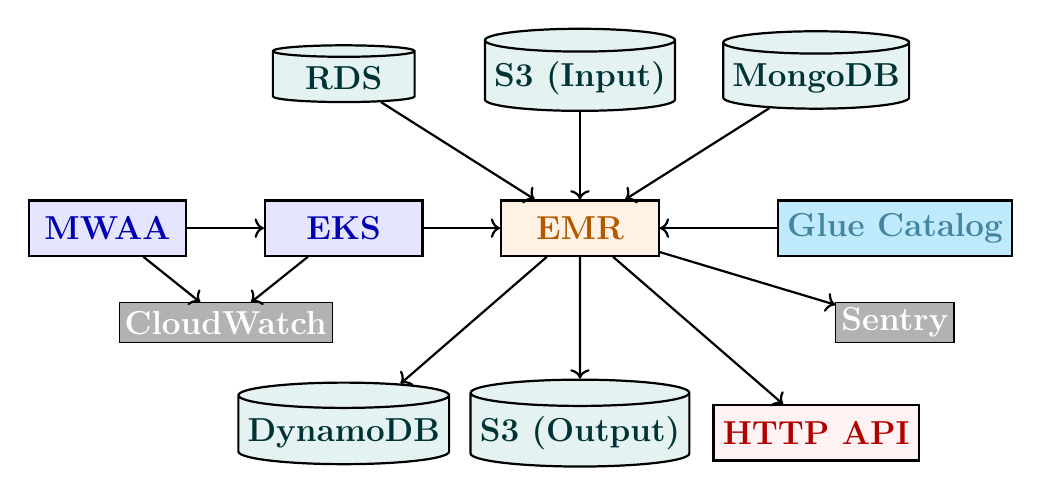
\begin{tikzpicture}[
    font=\sffamily,
    node distance=12mm,
% 노드 스타일
dist/.style={
    draw,
    rectangle,
    minimum width=2cm,
    minimum height=0.7cm,
    thick,
    fill=orange!10,
    font=\large\bfseries,
    text=orange!70!black,
},
orchestration/.style={
    draw,
    rectangle,
    minimum width=2cm,
    minimum height=0.7cm,
    thick,
    fill=blue!10,
    font=\large\bfseries,
    text=blue!70!black,
},
compute/.style={
    draw,
    rectangle,
    minimum width=2cm,
    minimum height=0.7cm,
    thick,
    fill=red!5!white,
    font=\large\bfseries,
    text=red!70!black,
},
catalog/.style={
    draw,
    rectangle,
    minimum width=2cm,
    minimum height=0.7cm,
    thick,
    fill=cyan!25,
    font=\large\bfseries,
    text=cyan!60!black,
},
storage/.style={
    draw,
    cylinder,
    shape border rotate=90,
    aspect=0.12,
    minimum width=1.8cm,
    minimum height=0.5cm,
    thick,
    fill=teal!10,
    font=\large\bfseries,
    text=teal!40!black,
},
monitor/.style={
    draw,
    rectangle,
    minimum width=0.8cm,
    minimum height=0.5cm,
    fill=gray!60,
    font=\bfseries\large,
    text=white,
    inner sep=2pt,
},
myarrow/.style={thick,->},
]
% Orchestration
\node[orchestration] (mwaa)   at (0,  1.5)  {MWAA};
\node[orchestration] (eks)    at (3,  1.5)  {EKS};
\node[monitor]     (cw)       at (1.5, 0.3)   {CloudWatch};

\node[dist]     (emr)      at (6,  1.5)  {EMR};

\node[catalog]     (glue)     at (10,  1.5)  {Glue Catalog};
% --- input
\node[storage]     (rds)      at (3,  3.4)    {RDS};
\node[storage]     (mongodb)  at (6,  3.4)    {S3 (Input)};
\node[storage]     (s3in)     at (9,  3.4)    {MongoDB};
% --- output
\node[storage]     (dynamodb) at (3, -1.1)  {DynamoDB};
\node[storage]     (s3out)    at (6, -1.1)    {S3 (Output)};
\node[compute]     (http)     at (9, -1.1) {HTTP API};

\node[monitor]     (sentry)   at (10,  0.3)   {Sentry};
% Edges
\draw[myarrow] (mwaa) -- (eks);
\draw[myarrow] (mwaa) -- (cw);
\draw[myarrow] (eks)  -- (cw);
\draw[myarrow] (eks)  -- (emr);
\draw[myarrow] (rds)     -- (emr);
\draw[myarrow] (glue)   -- (emr);
\draw[myarrow] (mongodb) -- (emr);
\draw[myarrow] (s3in)    -- (emr);
\draw[myarrow] (emr) -- (dynamodb);
\draw[myarrow] (emr) -- (s3out);
\draw[myarrow] (emr) -- (http);
\draw[myarrow] (emr) -- (sentry);
\end{tikzpicture}
}
\end{figure}

    \vspace{3mm}
    
    \textbf{주요 성과}:
        \begin{itemize}
            \item 기존 Jenkins Groovy 스크립트를 Python 기반 Airflow Operator로 전환하여 언어,플랫폼 일관성 확보, 코드 리뷰·테스트 자동화 적용으로 개발 생산성 향상
        \end{itemize}
    
    }
    \resumeSubProjectListStart
    \resumeSubProject{\textbf{스케줄러 전환: Jenkins → Airflow}}
    {
    
    기존 Jenkins Groovy 스크립트를 Python 기반 Airflow Operator 및 Sensor로 전환하여  
    언어,플랫폼 일관성을 확보하고, Airflow(Amazon MWAA) DAG로 모든 스케줄링을 통합하였습니다.
        \vspace{1mm}
        
        \textbf{사용한 기술}: Amazon MWAA, Python, Amazon EKS, Amazon Cloudwatch
        \vspace{2mm}
    }
    
    \resumeSubProject{\textbf{데이터 적재 자동화 및 모니터링 시스템 구축}}
    {
    
    Amazon S3를 데이터 레이크로 구축하고 AWS Glue Catalog와 연동하여 메타데이터 관리를 체계화했습니다. CloudWatch를 활용해 Amazon MWAA 및 EKS 클러스터 모니터링 시스템을 구현하고, Airflow DAG을 작성하여 자동화된 데이터 파이프라인을 운영하였습니다. 또한 Spark on EMR 작업 중 장애 발생 시 Sentry로 에러를 실시간 레포팅하도록 설정하였습니다.  

        \vspace{1mm}
        \textbf{사용한 기술}: Amazon Glue Catalog, Amazon MWAA, Amazon EKS, Amazon CloudWatch, Sentry 
        \vspace{2mm}
    }
    
    \resumeSubProject{\textbf{DynamoDB 입수 파이프라인 운영}}
    {
    
    Apache Spark를 활용하여 사용자 추천 데이터의 DynamoDB 입수 파이프라인을 설계 및 운영, 실시간 데이터 처리와 안정적인 API 서빙 환경을 구축하였습니다.

    \vspace{1mm}
    \textbf{사용한 기술}: Apache Spark, Amazon DynamoDB, Scala
    \vspace{2mm}
    }

    \resumeSubProjectListEnd

    %---------------- 서브 프로젝트 End

    \textbf{문제 해결(링크)}:
        \begin{itemize}
            \item \href{https://superhuman54.github.io/posts/conflict-between-emr-and-aws-sdk/}{Amazon EMR 6.12와 AWS Java SDK 충돌 문제}
            \item \href{https://superhuman54.github.io/posts/low-throughput-for-writing-to-dynamodb/}{Spark에서 DynamoDB 쓰기 성능 저하 문제}
            \item \href{https://superhuman54.github.io/posts/fail-to-releases-pods-on-the-same-k8s/}{공유 Kubernetes 클러스터에서 Airflow Pod 중복 생성 및 회수 실패 문제}
            \item \href{https://superhuman54.github.io/posts/failed-to-release-completed-pod/}{Amazon MWAA에서 Kubernetes Pod 회수 실패 문제}
        \end{itemize}
    
    %---------------- 트러블슛 End

  \resumeProjectListEnd


%-------------------------------------------
\section{\textbf{5. 추천 데이터 HTTP 서버 구축과 운영}}
  \resumeProjectListStart
    \resumeProject
    {\textbf{소속}: 드림어스컴퍼니} {}
    
    {\textbf{주요 내용}:
    기존 Flask 기반 HTTP 서버를 I/O 바운드 작업에 최적화된 FastAPI로 전환하였습니다. DynamoDB 조회가 많은 환경에서 FastAPI의 비동기 처리 덕분에 응답 지연 시간이 Flask의 약 500ms에서 FastAPI는 평균 120ms로 약 76\% 감소하여 처리 속도와 동시 처리 성능이 대폭 개선되었습니다. 또한, 타입 힌팅과 \href{https://python-dependency-injector.ets-labs.org/}{Dependency Injector} 도입으로 코드 품질과 유지보수성도 향상시켰습니다.
    
    \textbf{주요 성과}:
    \begin{itemize}
        \item 기존 Flask 대비 비동기 처리 기반 FastAPI 도입으로 API 요청 지연시간 76\% 감축 및 동시성 향상
        \item 타입 힌팅 적용과 Dependency Injection으로 코드 안정성과 유지보수성 강화
    \end{itemize}
    }

    \resumeSubProject{\textbf{FastAPI 전환 및 코드 품질 개선}}
    {
    
    기존 Flask 기반 HTTP 서버를 I/O 바운드 작업에 최적화된 FastAPI로 전환하면서, DynamoDB와 같은 외부 API 조회가 대량 발생하는 환경에서 응답 시간과 처리량이 향상되었습니다. FastAPI의 비동기 처리 및 타입 힌팅 덕분에 병목이 감소하며 전체 API 서버 성능이 크게 개선되었습니다. 또한, Dependency Injector를 활용해 코드 품질과 유지보수성 또한 강화했습니다.

    \vspace{1mm}
    \textbf{사용한 기술}: Python3.9, FastAPI, Dependency Injector, Amazon DynamoDB
    \vspace{2mm}
    }

    

  \resumeProjectListEnd

  
\end{document}